\subsection*{Elaborated sequential characterization design}

\begin{figure}
\centering
\tikzstyle{dot} = [draw,shape=circle,fill=black, scale =.2]
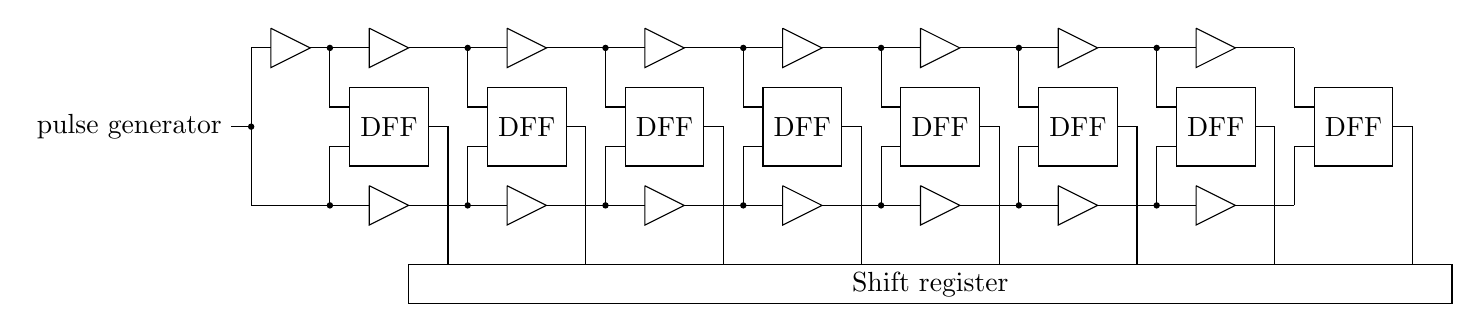
\begin{tikzpicture}
% one block
\draw  (1.75,0.5) rectangle (2.75,-0.5)node[pos=.5]{DFF};
\draw (2,1.25)-- (2.5,1) -- (2,0.75) -- (2,1.25);
\draw (2,-0.75)-- (2.5,-1) -- (2,-1.25) -- (2,-0.75);
\draw (2,1) -- (1.25,1);
\draw (2,-1) -- (0.5,-1);
\draw (1.75,0.25) -| (1.5,1);
\draw (1.75,-0.25) -| (1.5,-1);
\draw (3,-1.75) |- (2.75,0);

% one block
\draw  (3.5,0.5) rectangle (4.5,-0.5)node[pos=.5]{DFF};
\draw (3.75,1.25)-- (4.25,1) -- (3.75,0.75) -- (3.75,1.25);
\draw (3.75,-0.75)-- (4.25,-1) -- (3.75,-1.25) -- (3.75,-0.75);
\draw (3.75,1) -- (2.5,1);
\draw (3.75,-1) -- (2.5,-1);
\draw (3.5,0.25) -| (3.25,1);
\draw (3.5,-0.25) -| (3.25,-1);
\draw (4.75,-1.75) |- (4.5,0);

% one block
\draw  (5.25,0.5) rectangle (6.25,-0.5)node[pos=.5]{DFF};
\draw (5.5,1.25)-- (6,1) -- (5.5,0.75) -- (5.5,1.25);
\draw (5.5,-0.75)-- (6,-1) -- (5.5,-1.25) -- (5.5,-0.75);
\draw (5.5,1) -- (4.25,1);
\draw (5.5,-1) -- (4.25,-1);
\draw (5.25,0.25) -| (5,1);
\draw (5.25,-0.25) -| (5,-1);
\draw (6.5,-1.75) |- (6.25,0);

% one block
\draw  (7,0.5) rectangle (8,-0.5)node[pos=.5]{DFF};
\draw (7.25,1.25)-- (7.75,1) -- (7.25,0.75) -- (7.25,1.25);
\draw (7.25,-0.75)-- (7.75,-1) -- (7.25,-1.25) -- (7.25,-0.75);
\draw (7.25,1) -- (6,1);
\draw (7.25,-1) -- (6,-1);
\draw (7,0.25) -| (6.75,1);
\draw (7,-0.25) -| (6.75,-1);
\draw (8.25,-1.75) |- (8,0);

% one block
\draw  (8.75,0.5) rectangle (9.75,-0.5)node[pos=.5]{DFF};
\draw (9,1.25)-- (9.5,1) -- (9,0.75) -- (9,1.25);
\draw (9,-0.75)-- (9.5,-1) -- (9,-1.25) -- (9,-0.75);
\draw (9,1) -- (7.75,1);
\draw (9,-1) -- (7.75,-1);
\draw (8.75,0.25) -| (8.5,1);
\draw (8.75,-0.25) -| (8.5,-1);
\draw (10,-1.75) |- (9.75,0);

% one block
\draw  (10.5,0.5) rectangle (11.5,-0.5)node[pos=.5]{DFF};
\draw (10.75,1.25)-- (11.25,1) -- (10.75,0.75) -- (10.75,1.25);
\draw (10.75,-0.75)-- (11.25,-1) -- (10.75,-1.25) -- (10.75,-0.75);
\draw (10.75,1) -- (9.5,1);
\draw (10.75,-1) -- (9.5,-1);
\draw (10.5,0.25) -| (10.25,1);
\draw (10.5,-0.25) -| (10.25,-1);
\draw (11.75,-1.75) |- (11.5,0);

% one block
\draw  (12.25,0.5) rectangle (13.25,-0.5)node[pos=.5]{DFF};
\draw (12.5,1.25)-- (13,1) -- (12.5,0.75) -- (12.5,1.25);
\draw (12.5,-0.75)-- (13,-1) -- (12.5,-1.25) -- (12.5,-0.75);
\draw (12.5,1) -- (11.25,1);
\draw (12.5,-1) -- (11.25,-1);
\draw (12.25,0.25) -| (12,1);
\draw (12.25,-0.25) -| (12,-1);
\draw (13.5,-1.75) |- (13.25,0);

% one block
\draw  (14,0.5) rectangle (15,-0.5)node[pos=.5]{DFF};
\draw (13.75,1) -- (13,1);
\draw (13.75,-1) -- (13,-1);
\draw (14,0.25) -| (13.75,1);
\draw (14,-0.25) -| (13.75,-1);
\draw (15.25,-1.75) |- (15,0);

%other things
\draw (0.75,1.25) -- (1.25,1) -- (0.75,0.75) -- (0.75,1.25);
\draw (0.5,-1) |- (0.75,1);
\draw (0.25,0) -- (0.5,0);

%lots of dots
\node [dot] at (1.5,1) {};
\node [dot] at (3.25,1) {};
\node [dot] at (5,1) {};
\node [dot] at (6.75,1) {};
\node [dot] at (8.5,1) {};
\node [dot] at (10.25,1) {};
\node [dot] at (12,1) {};
\node [dot] at (12,-1) {};
\node [dot] at (10.25,-1) {};
\node [dot] at (8.5,-1) {};
\node [dot] at (6.75,-1) {};
\node [dot] at (5,-1) {};
\node [dot] at (3.25,-1) {};
\node [dot] at (1.5,-1) {};
\node [dot] at (0.5,0) {};

\draw  (2.5,-1.75) rectangle (15.75,-2.25)node[pos=.5]{Shift register};
\node [anchor=east] at (0.25,0) {pulse generator};
\end{tikzpicture}
\end{figure}